\documentclass[10pt]{article}
\usepackage[margin=0.75in]{geometry}\usepackage[T1]{fontenc}\usepackage{tikz,url}
\begin{document}\section*{Standalone Lean launcher exit propagation}
\textbf{Five fixed instrument controls; independent review pending.}

The previous helper records native Lean failures but returns success from its own process. A new helper revision now propagates native failure and returns exit 2 when local source/module bindings change during an otherwise successful invocation. Historical helper snapshots and theorem receipts are preserved.

\begin{center}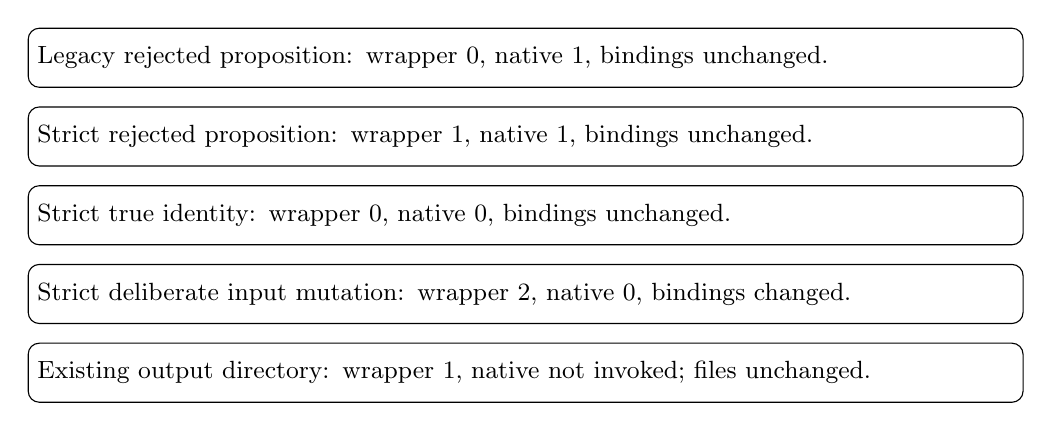
\begin{tikzpicture}[every node/.style={draw,rounded corners,align=left,text width=12.4cm,minimum height=0.75cm,font=\small}]
\node at (0,0) {Legacy rejected proposition: wrapper 0, native 1, bindings unchanged.};
\node at (0,-1) {Strict rejected proposition: wrapper 1, native 1, bindings unchanged.};
\node at (0,-2) {Strict true identity: wrapper 0, native 0, bindings unchanged.};
\node at (0,-3) {Strict deliberate input mutation: wrapper 2, native 0, bindings changed.};
\node at (0,-4) {Existing output directory: wrapper 1, native not invoked; files unchanged.};
\end{tikzpicture}\end{center}
\subsection*{Method and observations}
The true proposition is $1=1$ over natural numbers. The rejected proposition is $0=1$. A deliberate instrument-only \texttt{\#eval} writes this fresh packet's marker file to test the binding-mismatch path; it is not theorem evidence. The marker's original and changed bytes are retained. The stale-directory control hashes the prior results before and after attempted reuse.

The new helper retains the native timeout of 120 seconds, one Lean thread and 4096 MiB memory setting. Its logic chooses the native nonzero exit first; otherwise it chooses zero for unchanged bindings and two for changed bindings. Each fixed outcome matched its expected process status. No timing or statistical inference is made from these controls.
\subsection*{Evidence and scope}
\texttt{results.json} contains the typed control outcomes. Each native invocation has command, stdout, stderr, source hash and before/after input inventories. \texttt{strict\_check.py} and \texttt{legacy\_check.py} preserve both versions. \texttt{status.json} records scope and review status; \texttt{flow.svg} is the editable companion diagram.

The historical final theorem checks were assessed using native receipts and unchanged bindings; this process-status defect does not change those recorded outcomes. Named-theorem axiom audits, independent source-fidelity review and canonical integration are separate tasks. No scientific workload was executed.

Source review: the retained standalone helper and Python's documented subprocess return-code contract (\url{https://docs.python.org/3/library/subprocess.html}). The exact reproduction and correction are bound in this packet. Next: independently review the launcher and use the corrected revision for subsequent standalone checks.
\end{document}
